% CSE 816 Mini-Project report. Build: pdflatex report.tex (run twice for references)
\documentclass[10pt,a4paper]{article}

\usepackage[a4paper,margin=16mm,top=13mm,bottom=15mm]{geometry}
\usepackage[T1]{fontenc}
\usepackage{lmodern}
\usepackage{microtype}
\usepackage{graphicx}
\usepackage{xcolor}
\usepackage{tabularx,booktabs,array}
\usepackage[hidelinks]{hyperref}
\usepackage{enumitem}
\usepackage[font=footnotesize,labelfont=bf,skip=3pt]{caption}
\usepackage{float}
\usepackage{titlesec}
\usepackage{tikz}
\usetikzlibrary{arrows.meta}

\definecolor{accent}{HTML}{0B5CAD}
\definecolor{muted}{HTML}{57606A}
\definecolor{okfill}{HTML}{E9F6EC}
\definecolor{okline}{HTML}{1A7F37}
\definecolor{boxfill}{HTML}{EEF4FB}
\definecolor{mailfill}{HTML}{FDECEC}
\definecolor{mailline}{HTML}{CF222E}

\titleformat{\section}{\large\bfseries}{\thesection.}{0.4em}{}
\titlespacing*{\section}{0pt}{1.5ex}{0.6ex}
\setlist{nosep,leftmargin=1.4em,topsep=2pt}
\setlength{\parindent}{0pt}
\setlength{\parskip}{3.5pt}
\setlength{\fboxsep}{0pt}
\newcommand{\cmd}[1]{\texttt{#1}}
\newcommand{\shot}[2][]{\fbox{\includegraphics[#1]{#2}}}% frame adds 0.8pt; widths below allow for it
\newcommand{\sep}{\quad\textcolor{muted}{|}\quad}

\begin{document}

\begin{center}
{\Large\bfseries End-to-End CI/CD Pipeline for a Calculator REST API\par}
\vspace{3pt}
{\small Subhash H\par}
{\small GitHub: \href{https://github.com/Subhashhari/calculator-devops}{\textcolor{accent}{\texttt{github.com/Subhashhari/calculator-devops}}}\par}
{\small Docker Hub: \href{https://hub.docker.com/r/subhashh2005/calculator-api}{\textcolor{accent}{\texttt{hub.docker.com/r/subhashh2005/calculator-api}}}\par}
\end{center}

\section{Overview and pipeline architecture}
A Spring Boot calculator API is taken from a pull request to a verified, load-balanced deployment with no manual step.
Merging into \cmd{main} makes GitHub send a webhook to Jenkins. Jenkins runs the declarative pipeline in the repository's \cmd{Jenkinsfile}: it builds and tests the code, pushes a new image to Docker Hub, redeploys the Docker Compose stack, checks that the stack is healthy, and emails the result.

\begin{figure}[H]
\centering
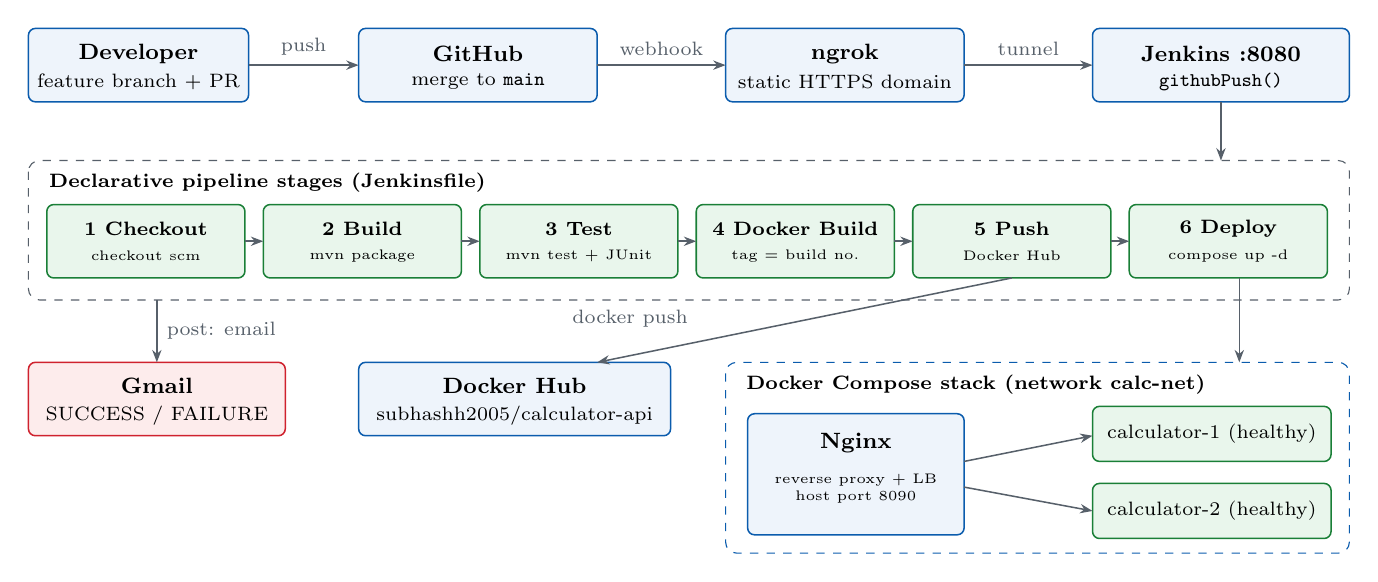
\begin{tikzpicture}[x=0.0233cm,y=-0.0233cm,
    box/.style={draw=accent,fill=boxfill,rounded corners=2.5pt,line width=0.55pt},
    stage/.style={draw=okline,fill=okfill,rounded corners=2.5pt,line width=0.55pt},
    mail/.style={draw=mailline,fill=mailfill,rounded corners=2.5pt,line width=0.55pt},
    group/.style={draw=muted,dashed,rounded corners=4pt},
    arr/.style={-{Stealth[length=4.5pt]},draw=muted,line width=0.55pt},
    lbl/.style={font=\scriptsize\color{muted}},
    t/.style={font=\footnotesize\bfseries},
    s/.style={font=\scriptsize}]
  % trigger path
  \draw[box] (20,14) rectangle (140,54);   \node[t] at (80,28) {Developer};     \node[s] at (80,43) {feature branch + PR};
  \draw[box] (200,14) rectangle (330,54);  \node[t] at (265,28) {GitHub};       \node[s] at (265,43) {merge to \texttt{main}};
  \draw[box] (400,14) rectangle (530,54);  \node[t] at (465,28) {ngrok};        \node[s] at (465,43) {static HTTPS domain};
  \draw[box] (600,14) rectangle (740,54);  \node[t] at (670,28) {Jenkins :8080}; \node[s] at (670,43) {\texttt{githubPush()}};
  \draw[arr] (140,34) -- node[lbl,above]{push} (200,34);
  \draw[arr] (330,34) -- node[lbl,above]{webhook} (400,34);
  \draw[arr] (530,34) -- node[lbl,above]{tunnel} (600,34);
  \draw[arr] (670,54) -- (670,86);
  % stages
  \draw[group] (20,86) rectangle (740,162);
  \node[font=\scriptsize\bfseries,anchor=west] at (26,98) {Declarative pipeline stages (Jenkinsfile)};
  \foreach \x/\a/\b in {30/1 Checkout/checkout scm, 148/2 Build/mvn package, 266/3 Test/mvn test + JUnit,
                        384/4 Docker Build/tag = build no., 502/5 Push/Docker Hub, 620/6 Deploy/compose up -d} {
    \draw[stage] (\x,110) rectangle ({\x+108},150);
    \node[font=\scriptsize\bfseries] at ({\x+54},123) {\a};
    \node[font=\tiny] at ({\x+54},138) {\b};
  }
  \foreach \x in {138,256,374,492,610} \draw[arr] (\x,130) -- ({\x+10},130);
  % outputs
  \draw[mail] (20,196) rectangle (160,236);  \node[t] at (90,209) {Gmail};       \node[s] at (90,225) {SUCCESS / FAILURE};
  \draw[box] (200,196) rectangle (370,236);  \node[t] at (285,209) {Docker Hub};  \node[s] at (285,225) {subhashh2005/calculator-api};
  \draw[arr] (90,162) -- node[lbl,right]{post: email} (90,196);
  \draw[arr] (556,150) -- (330,196);
  \node[lbl] at (348,172) {docker push};
  % compose stack
  \draw[group,draw=accent] (400,196) rectangle (740,300);
  \node[font=\scriptsize\bfseries,anchor=west] at (406,208) {Docker Compose stack (network calc-net)};
  \draw[box] (412,224) rectangle (530,290);
  \node[t] at (471,240) {Nginx};
  \node[font=\tiny,align=center] at (471,265) {reverse proxy + LB\\host port 8090};
  \draw[stage] (600,220) rectangle (730,250);  \node[s] at (665,235) {calculator-1 (healthy)};
  \draw[stage] (600,262) rectangle (730,292);  \node[s] at (665,277) {calculator-2 (healthy)};
  \draw[arr] (530,250) -- (600,236);
  \draw[arr] (530,264) -- (600,277);
  \draw[arr] (680,150) -- (680,196);
\end{tikzpicture}
\caption{Pipeline architecture. A merged PR reaches Jenkins through a GitHub webhook over an ngrok tunnel. The six stages publish \cmd{:<build no.>} to Docker Hub and redeploy two API replicas behind Nginx, and the result is emailed.}
\label{fig:arch}
\end{figure}

\section{Application and testing}
The service uses Spring Boot 4.1 on Java 21 with Maven, and is layered as controller $\to$ service $\to$ DTO.
The endpoints \cmd{GET /api/v1/add}, \cmd{/subtract}, \cmd{/multiply} and \cmd{/divide} take query parameters \cmd{a} and \cmd{b}. For example, \cmd{add?a=2\&b=3} returns
\cmd{\{"operation":"add","a":2.0,"b":3.0,"result":5.0\}}.
A single \cmd{@RestControllerAdvice} turns every client error into HTTP~400 with a structured body (\cmd{timestamp}, \cmd{status}, \cmd{error}, \cmd{message}, \cmd{path}). It covers division by zero, a missing or non-numeric parameter, NaN/Infinity, and an overflowing result.
Division by zero needs an explicit check, because with \cmd{double}, \cmd{1/0} silently yields \cmd{Infinity}. Spring Boot Actuator exposes \cmd{/actuator/health}, which every health check in the system uses.

There are 28 JUnit~5 tests. \cmd{CalculatorServiceTest} has 19 unit tests, mostly parameterized, covering every operation, divide-by-zero, non-finite input and overflow. \cmd{CalculatorControllerTest} has 9 integration tests: \cmd{@SpringBootTest} with MockMvc hits the real endpoints, the three 400 cases and the health probe.
\cmd{mvn test} writes JUnit XML to \cmd{target/surefire-reports}, and Jenkins publishes it.

\section{CI/CD pipeline (Jenkinsfile)}
\begin{enumerate}
  \item \textbf{Checkout:} \cmd{checkout scm} of the merged commit. The implicit checkout is disabled so this stage owns it.
  \item \textbf{Build:} \cmd{mvn -B clean package -DskipTests} using the Jenkins-managed tools \cmd{JDK-21} and \cmd{Maven-3.9}.
  \item \textbf{Test:} \cmd{mvn -B test}, then \cmd{junit 'target/surefire-reports/*.xml'}. A failing test fails the stage, and every later stage is skipped.
  \item \textbf{Docker Build:} builds the multi-stage image as \cmd{subhashh2005/calculator-api:}\textit{build-number} and \cmd{:latest}.
  \item \textbf{Push:} \cmd{credentials('dockerhub-creds')} exposes a masked user and access token. The stage runs \cmd{docker login --password-stdin} and pushes both tags. The Docker Hub user name comes from the credential, so it is not hard-coded anywhere.
  \item \textbf{Deploy:} \cmd{docker compose up -d --wait --remove-orphans} with \cmd{IMAGE\_TAG} set to the build number. \cmd{--wait} fails the stage unless every health check passes. A \cmd{curl} smoke test through Nginx then checks \cmd{/actuator/health} and that \cmd{2+3} returns \cmd{5.0}.
\end{enumerate}
\textbf{Trigger.} \cmd{githubPush()} fires on the webhook. GitHub cannot reach \cmd{localhost:8080}, so the webhook targets a static ngrok domain that tunnels to Jenkins. \cmd{pollSCM('H/5 * * * *')} remains as a fallback.
Build \#4 was \emph{``Started by GitHub push''} within seconds of merging PR \#1 (Fig.~\ref{fig:green}).
\textbf{Notifications.} The \cmd{post} block sends a SUCCESS email (build number, image tag, link) or a FAILURE email with \cmd{build.log} attached, through Gmail SMTP over SSL with an app password. The recipients are set in Jenkins, not in the repository.
\textbf{Idempotence.} \cmd{disableConcurrentBuilds()}, the fixed Compose project name \cmd{calculator}, and \cmd{up -d} (which recreates only changed containers) make re-runs safe. Nginx stayed up through every redeploy (Fig.~\ref{fig:ps}).

\begin{figure}[H]
\centering
\begin{minipage}[t]{0.495\linewidth}\vspace{0pt}\centering
  \shot[width=0.99\linewidth,trim=0 490 0 0,clip]{build_4.png}
  \caption{Build \#4, started by GitHub push: all six stages and the post actions are green.}\label{fig:green}
\end{minipage}\hfill
\begin{minipage}[t]{0.495\linewidth}\vspace{0pt}\centering
  \shot[width=0.99\linewidth,trim=0 552 0 0,clip]{build_5.png}
  \caption{Build \#5 (deliberately broken test, PR \#2): Test fails, so Docker Build, Push and Deploy are skipped.}\label{fig:red}
\end{minipage}

\vspace{5pt}
\begin{minipage}[t]{0.495\linewidth}\vspace{0pt}\centering
  \shot[width=0.86\linewidth,trim=0 192 1243 0,clip]{build_4_mail.png}
  \caption{SUCCESS email for build \#4.}\label{fig:mailok}
\end{minipage}\hfill
\begin{minipage}[t]{0.495\linewidth}\vspace{0pt}\centering
  \shot[width=0.86\linewidth,trim=0 192 1243 0,clip]{build_5_mail.png}
  \caption{FAILURE email for build \#5, with the console log attached.}\label{fig:mailfail}
\end{minipage}
\end{figure}

\section{Containerization (Dockerfile)}
The \textbf{build stage} (\cmd{maven:3.9-eclipse-temurin-21}) copies \cmd{pom.xml} first and runs \cmd{mvn dependency:go-offline} before adding \cmd{src/}. Dependencies therefore form a cached layer, and a code-only change rebuilds only the last step.
The \textbf{runtime stage} (\cmd{eclipse-temurin:21-jre-alpine}) copies just the JAR and runs it as the non-root user \cmd{app}. It declares \cmd{EXPOSE 8080} and has a \cmd{HEALTHCHECK} that calls \cmd{/actuator/health} with BusyBox \cmd{wget}.
The image is about 95\,MB compressed. \cmd{JAVA\_OPTS} is honoured by an \cmd{exec java} entrypoint, and \cmd{.dockerignore} keeps \cmd{target/}, \cmd{.git}, IDE files and \cmd{.env} out of the build context.
A single \cmd{docker run -p 8085:8080 subhashh2005/calculator-api} answers on the mapped port.

\section{Compose deployment and verification}
\cmd{docker-compose.yml} defines:
\begin{itemize}
  \item the bridge network \cmd{calc-net};
  \item the \cmd{calculator} service with \textbf{two replicas}, an Actuator health check, \cmd{restart: unless-stopped}, and the environment variables \cmd{SPRING\_PROFILES\_ACTIVE} and \cmd{JAVA\_OPTS};
  \item an \textbf{Nginx} reverse proxy, the only published port (8090), which starts only once the API is healthy and has its own health check.
\end{itemize}
The image and tag are parameters (\cmd{DOCKER\_IMAGE}, \cmd{IMAGE\_TAG}), so Jenkins deploys exactly the image it pushed.
Nginx uses \cmd{upstream \{ server calculator:8080 resolve; \}} with Docker's DNS (\cmd{127.0.0.11}). It therefore round-robins across both replicas and follows their new IPs after a redeploy, and the \cmd{X-Upstream} response header shows which replica answered.
The deployment was verified with \cmd{docker ps}, calls to every endpoint through Nginx including the 400 cases, and the redeploy from \cmd{:4} to \cmd{:6}.

\begin{figure}[H]
\centering
\shot[width=0.99\linewidth,trim=0 0 727 0,clip]{docker-ps.png}
\caption{\cmd{docker ps} after build \#6: two healthy replicas running \cmd{:6} and the Nginx proxy on host port 8090. Nginx was not recreated by the redeploy.}\label{fig:ps}
\end{figure}
\begin{figure}[H]
\centering
\shot[width=0.99\linewidth,trim=0 0 913 0,clip]{curl_responses.png}
\caption{API responses through Nginx: the four operations, three HTTP~400 errors and the health endpoint.}\label{fig:curl}
\end{figure}
\begin{figure}[H]
\centering
\shot[width=0.55\linewidth]{load_balancing.png}
\caption{The \cmd{X-Upstream} header alternates between the two replicas, showing round-robin load balancing.}\label{fig:lb}
\end{figure}

\section{Version control}
\cmd{main} has 18 commits: 15 Conventional-Commit changes (\cmd{feat}, \cmd{test}, \cmd{build}, \cmd{ci}, \cmd{docs}, \cmd{fix}, \cmd{chore}) and 3 pull-request merges.
\textbf{PR \#1} (\cmd{docs/dockerhub-link}) was the first webhook-triggered deploy. \textbf{PR \#2} (\cmd{test/failing-build}) deliberately broke a test to prove that a failure blocks deployment. \textbf{PR \#3} reverted it, and build \#6 went green.
\cmd{.gitignore} excludes \cmd{target/}, IDE files, logs and \cmd{.env}. The Docker Hub token and Gmail app password exist only in the Jenkins credential store.

\section{Challenges faced}
\begin{tabularx}{\linewidth}{@{}>{\raggedright\arraybackslash}p{0.25\linewidth}>{\raggedright\arraybackslash}X@{}}
\toprule
\textbf{Challenge} & \textbf{Cause and resolution}\\
\midrule
Jenkins \cmd{apt} install hung & IPv6 connections to \cmd{pkg.jenkins.io} time out on this network. Used \cmd{wget -4} and \cmd{apt -o Acquire::ForceIPv4=true}, and added \cmd{-Djava.net.preferIPv4Stack=true} to Jenkins with a systemd override so plugin and Maven downloads work.\\
\cmd{NO\_PUBKEY 7198F4B714ABFC68} & The Jenkins repository signing key had been rotated. Switched to \cmd{jenkins.io-2026.key} after checking that its fingerprint matched the missing key.\\
Parent POM not found & Spring Initializr labels the version \cmd{4.1.2.RELEASE}, but the Maven artifact is \cmd{4.1.2}. Fixed the parent version.\\
\cmd{@AutoConfigureMockMvc} not found & Spring Boot 4 moved the MockMvc auto-configuration into \cmd{spring-boot-starter-webmvc-test} (package \cmd{org.springframework.boot.webmvc.test.autoconfigure}).\\
First build failed at compile time & \emph{``Tool type jdk does not have an install of JDK-21''}: the tool had been registered as \cmd{jdk-21}, and names are case-sensitive. Renamed it. The Jenkinsfile itself had been checked earlier with Jenkins' declarative linter.\\
Nginx sent every request to one replica & A variable in \cmd{proxy\_pass} re-resolved DNS but stuck to one address. An \cmd{upstream} with \cmd{server \dots{} resolve} (Nginx 1.28) balances both replicas and tracks new IPs.\\
Port 80 already in use & Another service holds port 80. Nginx is published on 8090, Jenkins keeps 8080, and the API replicas are not published at all.\\
GitHub cannot reach Jenkins & Jenkins runs on a laptop. An ngrok static domain forwards the webhook, and Poll SCM is kept as a fallback in case the tunnel is down.\\
\bottomrule
\end{tabularx}

\textbf{Demonstration.} Start the ngrok tunnel. Make a small change on a feature branch, open a PR and merge it. Then show Jenkins starting by itself, the six stages turning green, the new tag on Docker Hub, the SUCCESS email, and \cmd{docker ps} showing the replicas on the new tag while Nginx keeps serving.

\end{document}
